%%%%%%%%%%%%%%%%%%%%%%%%%%%%%%%%%%%%%%%%%%%%%%%%%%%%%%%%%%%%%%%%%%%%%%%%%%%
%% This file is part of the book
%%
%% Algorithmic Graph Theory
%% http://code.google.com/p/graph-theory-algorithms-book/
%%
%% Copyright (C) 2009--2011 Minh Van Nguyen <nguyenminh2@gmail.com>
%%
%% See the file COPYING for copying conditions.
%%%%%%%%%%%%%%%%%%%%%%%%%%%%%%%%%%%%%%%%%%%%%%%%%%%%%%%%%%%%%%%%%%%%%%%%%%%

\documentclass{article}

\usepackage{subfigure}
\usepackage{tikz}
\usetikzlibrary{external}
\usetikzlibrary{trees}
\tikzexternalize{construct-Huffman-tree}

\begin{document}

\begin{figure}
\subfigure[]{

\begin{tikzpicture}
[-,thick,%
  every node/.style={shape=rectangle,inner sep=1.5pt,draw,thick},%
  scale=0.5]
\scriptsize
\foreach \xcoord/\xval in {
  0/13, 1.5/2, 3/1, 4.5/19, 6/4, 7.5/5, 9/2, 10.5/7, 12/1, 13.5/3}
{
  \node at (\xcoord,0) {$\xval$};
}
\end{tikzpicture}
}
%%
%%
\qquad
\subfigure[]{
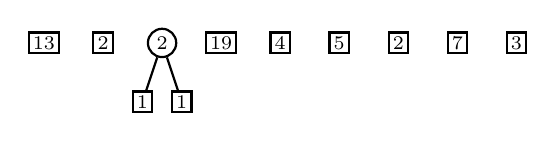
\begin{tikzpicture}
[-,thick,%
  every node/.style={shape=rectangle,inner sep=1.5pt,draw,thick},%
  scale=0.5]
\scriptsize
\node at (0,0) {$13$};
\node at (1.5,0) {$2$};
\node[shape=circle] at (3,0) {$2$}
  [sibling distance=1cm]
  child {node {$1$}}
  child {node {$1$}};
\node at (4.5,0) {$19$};
\node at (6,0) {$4$};
\node at (7.5,0) {$5$};
\node at (9,0) {$2$};
\node at (10.5,0) {$7$};
\node at (12,0) {$3$};
\end{tikzpicture}
}
%%
%%
\subfigure[]{
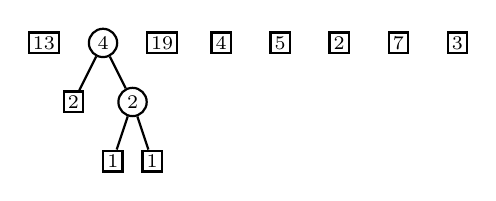
\begin{tikzpicture}
[-,thick,%
  every node/.style={shape=rectangle,inner sep=1.5pt,draw,thick},%
  scale=0.5]
\scriptsize
\node at (0,0) {$13$};
\node[shape=circle] at (1.5,0) {$4$}
  child {node {$2$}}
  child {node[shape=circle] {$2$}
    [sibling distance=1cm]
    child {node {$1$}}
    child {node {$1$}}};
\node at (3,0) {$19$};
\node at (4.5,0) {$4$};
\node at (6,0) {$5$};
\node at (7.5,0) {$2$};
\node at (9,0) {$7$};
\node at (10.5,0) {$3$};
\end{tikzpicture}
}
%%
%%
\qquad\qquad
\subfigure[]{
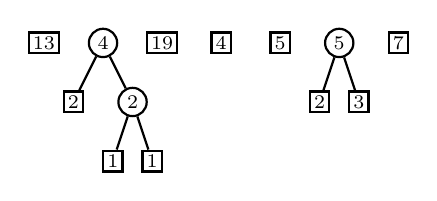
\begin{tikzpicture}
[-,thick,%
  every node/.style={shape=rectangle,inner sep=1.5pt,draw,thick},%
  scale=0.5]
\scriptsize
\node at (0,0) {$13$};
\node[shape=circle] at (1.5,0) {$4$}
  child {node {$2$}}
  child {node[shape=circle] {$2$}
    [sibling distance=1cm]
    child {node {$1$}}
    child {node {$1$}}};
\node at (3,0) {$19$};
\node at (4.5,0) {$4$};
\node at (6,0) {$5$};
\node[shape=circle] at (7.5,0) {$5$}
  [sibling distance=1cm]
  child {node {$2$}}
  child {node {$3$}};
\node at (9,0) {$7$};
\end{tikzpicture}
}
%%
%%
\subfigure[]{
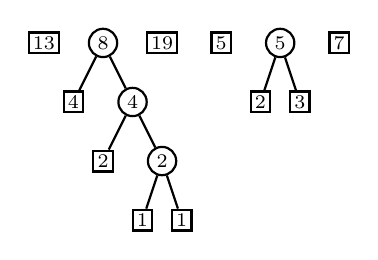
\begin{tikzpicture}
[-,thick,%
  every node/.style={shape=rectangle,inner sep=1.5pt,draw,thick},%
  scale=0.5]
\scriptsize
\node at (0,0) {$13$};
\node[shape=circle] at (1.5,0) {$8$}
  child {node {$4$}}
  child {node[shape=circle] {$4$}
    child {node {$2$}}
    child {node[shape=circle] {$2$}
      [sibling distance=1cm]
      child {node {$1$}}
      child {node {$1$}}}
  };
\node at (3,0) {$19$};
\node at (4.5,0) {$5$};
\node[shape=circle] at (6,0) {$5$}
  [sibling distance=1cm]
  child {node {$2$}}
  child {node {$3$}};
\node at (7.5,0) {$7$};
\end{tikzpicture}
}
%%
%%
\quad\qquad
\subfigure[]{
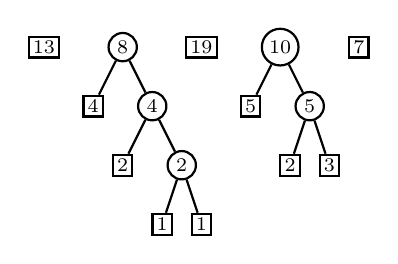
\begin{tikzpicture}
[-,thick,%
  every node/.style={shape=rectangle,inner sep=1.5pt,draw,thick},%
  scale=0.5]
\scriptsize
\node at (0,0) {$13$};
\node[shape=circle] at (2,0) {$8$}
  child {node {$4$}}
  child {node[shape=circle] {$4$}
    child {node {$2$}}
    child {node[shape=circle] {$2$}
      [sibling distance=1cm]
      child {node {$1$}}
      child {node {$1$}}}
  };
\node at (4,0) {$19$};
\node[shape=circle] at (6,0) {$10$}
  child {node {$5$}}
  child {node[shape=circle] {$5$}
    [sibling distance=1cm]
    child {node {$2$}}
    child {node {$3$}}
  };
\node at (8,0) {$7$};
\end{tikzpicture}
}
%%
%%
\qquad
\subfigure[]{
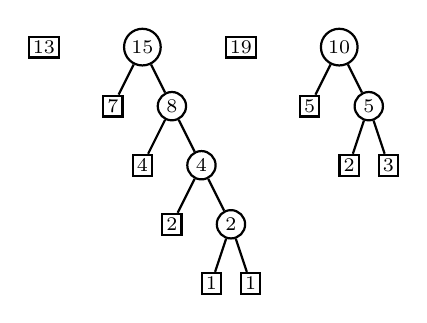
\begin{tikzpicture}
[-,thick,%
  every node/.style={shape=rectangle,inner sep=1.5pt,draw,thick},%
  scale=0.5]
\scriptsize
\node at (0,0) {$13$};
\node[shape=circle] at (2.5,0) {$15$}
  child {node {$7$}}
  child {node[shape=circle] {$8$}
    child {node {$4$}}
    child {node[shape=circle] {$4$}
      child {node {$2$}}
      child {node[shape=circle] {$2$}
        [sibling distance=1cm]
        child {node {$1$}}
        child {node {$1$}}}
    }
  };
\node at (5,0) {$19$};
\node[shape=circle] at (7.5,0) {$10$}
  child {node {$5$}}
  child {node[shape=circle] {$5$}
  [sibling distance=1cm]
    child {node {$2$}}
    child {node {$3$}}
  };
\end{tikzpicture}
}
%%
%%
\qquad\qquad
\subfigure[]{
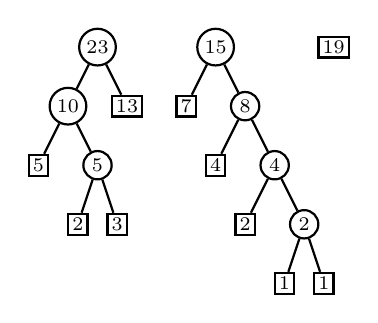
\begin{tikzpicture}
[-,thick,%
  every node/.style={shape=rectangle,inner sep=1.5pt,draw,thick},%
  scale=0.5]
\scriptsize
\node[shape=circle] at (0,0) {$23$}
  child {node[shape=circle] {$10$}
    child {node {$5$}}
    child {node[shape=circle] {$5$}
      [sibling distance=1cm]
      child {node {$2$}}
      child {node {$3$}}
    }
  }
  child {node {$13$}};
\node[shape=circle] at (3,0) {$15$}
  child {node {$7$}}
  child {node[shape=circle] {$8$}
    child {node {$4$}}
    child {node[shape=circle] {$4$}
      child {node {$2$}}
      child {node[shape=circle] {$2$}
        [sibling distance=1cm]
        child {node {$1$}}
        child {node {$1$}}}
    }
  };
\node at (6,0) {$19$};
\end{tikzpicture}
}
%%
%%
\qquad\quad
\subfigure[]{
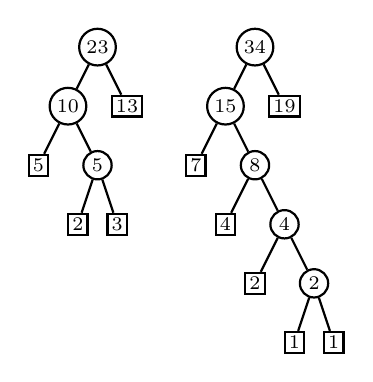
\begin{tikzpicture}
[-,thick,%
  every node/.style={shape=rectangle,inner sep=1.5pt,draw,thick},%
  scale=0.5]
\scriptsize
\node[shape=circle] at (0,0) {$23$}
  child {node[shape=circle] {$10$}
    child {node {$5$}}
    child {node[shape=circle] {$5$}
      [sibling distance=1cm]
      child {node {$2$}}
      child {node {$3$}}
    }
  }
  child {node {$13$}};
\node[shape=circle] at (4,0) {$34$}
  child {node[shape=circle] {$15$}
    child {node {$7$}}
    child {node[shape=circle] {$8$}
      child {node {$4$}}
      child {node[shape=circle] {$4$}
        child {node {$2$}}
        child {node[shape=circle] {$2$}
          [sibling distance=1cm]
          child {node {$1$}}
          child {node {$1$}}}
      }
    }
  }
  child {node {$19$}};
\end{tikzpicture}
}
%%
%%
\qquad\qquad
\subfigure[]{
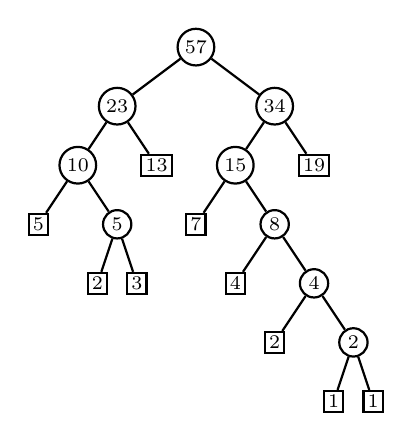
\begin{tikzpicture}
[-,thick,%
  every node/.style={shape=rectangle,inner sep=1.5pt,draw,thick},%
  scale=0.5]
\scriptsize
\node[shape=circle] {$57$}
  [sibling distance=4cm]
  child {node[shape=circle] {$23$}
    [sibling distance=2cm]
    child {node[shape=circle] {$10$}
      child {node {$5$}}
      child {node[shape=circle] {$5$}
        [sibling distance=1cm]
        child {node {$2$}}
        child {node {$3$}}
      }
    }
    child {node {$13$}}
  }
  child {node[shape=circle] {$34$}
    [sibling distance=2cm]
    child {node[shape=circle] {$15$}
      child {node {$7$}}
      child {node[shape=circle] {$8$}
        child {node {$4$}}
        child {node[shape=circle] {$4$}
          child {node {$2$}}
          child {node[shape=circle] {$2$}
            [sibling distance=1cm]
            child {node {$1$}}
            child {node {$1$}}}
        }
      }
    }
    child {node {$19$}}
  };
\end{tikzpicture}
}
\end{figure}

\end{document}
